\chapter{Kết quả và thảo luận}
\label{ch:results}

Chương này báo cáo kết quả chính trên bộ dữ liệu phân xưởng, ablation trên hai cách chia dữ liệu và kết quả trên AVA~v2.2. Số liệu trên dữ liệu phân xưởng và 39,1 mAP trên AVA~v2.2 thuộc mức bằng chứng E2 (hồ sơ thực nghiệm); số liệu của lần chạy trên tập con AVA thuộc mức E1 (\code{trainning.log}); số liệu từ công trình khác chỉ dùng để định vị khoảng hiệu năng (\cref{sec:reference}).

\section{Kết quả chính trên bộ dữ liệu phân xưởng}
\label{sec:main-results}

\Cref{tab:main-results} so sánh pipeline đầy đủ với các mô hình trong hồ sơ thực nghiệm, trên cách chia ngẫu nhiên của các lượt chạy ban đầu. Pipeline đề xuất đạt 89,83\% mAP, cao hơn mô hình mạnh nhất còn lại là FastViT3D-SA12 5,17 điểm và EfficientViT3D-b1 10,07 điểm; khoảng cách với YOWOv2-Nano (31,28 điểm) và SlowFast-R50 (60,56 điểm) lớn hơn nhiều. Khi bỏ ACRN, pipeline còn 83,60\%, tức ACRN đóng góp 6,23 điểm trong cặp lượt chạy này. Cấu hình không ACRN tương ứng A7; trung bình ba hạt giống của A7 và A8 trên S1 là 83,71\% và 89,60\% (\cref{tab:ablation-results}), rất gần hai lượt chạy trong hồ sơ.

\begin{table}[htbp]
\centering
\caption{So sánh mAP trên bộ dữ liệu phân xưởng (hồ sơ thực nghiệm, cách chia ngẫu nhiên)}
\label{tab:main-results}
\begin{tabularx}{\textwidth}{Xrr}
\toprule
\textbf{Mô hình} & \textbf{mAP (\%)} & \textbf{So với pipeline đầy đủ}\\
\midrule
SlowFast-R50 \cite{feichtenhofer2019slowfast} & 29,27 & $-60{,}56$\\
YOWOv2-Nano \cite{yang2023yowov2} & 58,55 & $-31{,}28$\\
EfficientViT3D-b1 \cite{cai2023efficientvit} & 79,76 & $-10{,}07$\\
Video Swin-T + Hybrid FGTN-Mamba (không ACRN) & 83,60 & $-6{,}23$\\
FastViT3D-SA12 \cite{vasu2023fastvit} & 84,66 & $-5{,}17$\\
\textbf{Video Swin-T + Hybrid FGTN-Mamba đa tỉ lệ + ACRN} & \textbf{89,83} & ---\\
\bottomrule
\end{tabularx}
\end{table}

Về chỉ số vận hành (\cref{tab:operating}), Precision và Recall tại ngưỡng 0,5 cùng bằng 81,82\%: tại điểm vận hành này, ở mức từng người và từng khung hình khóa, khoảng 18\% dự đoán dương là sai và khoảng 18\% hành vi thật bị bỏ sót. Ngưỡng theo lớp và logic theo track (\cref{sec:loss,sec:inference}) cho phép dịch điểm vận hành theo yêu cầu nghiệp vụ, ví dụ ưu tiên recall với \path{dangerous_action}. Tốc độ trên 20 khung hình/giây với khoảng 10~GB bộ nhớ GPU đáp ứng yêu cầu giám sát theo thời gian thực (M6); đây là thông lượng của mô hình, chưa gồm bộ phát hiện người và bộ đệm nhìn trước của quét hai chiều.

\begin{table}[htbp]
\centering
\caption{Chỉ số vận hành của pipeline đầy đủ trên bộ dữ liệu phân xưởng (hồ sơ thực nghiệm)}
\label{tab:operating}
\begin{tabularx}{\textwidth}{lX}
\toprule
\textbf{Chỉ số} & \textbf{Giá trị}\\
\midrule
mAP & 89,83\%\\
Precision / Recall tại ngưỡng 0,5 & 81,82\% / 81,82\%\\
Tốc độ xử lý; bộ nhớ GPU & Trên 20 khung hình/giây; khoảng 10~GB\\
Điều kiện đo & \canbosung{GPU, độ phân giải, kích thước lô; có tính bộ phát hiện người hay không}\\
\bottomrule
\end{tabularx}
\end{table}

\section{Ablation: đóng góp của từng thành phần}
\label{sec:ablation-results}

\Cref{tab:ablation-results} và \cref{fig:ablation} trình bày mAP của chín cấu hình A0--A8 (\cref{tab:ablation}); mỗi giá trị là trung bình ba hạt giống, trên hai cách chia S1 (ngẫu nhiên) và S2 (giữ riêng hai camera để kiểm tra).

\begin{table}[H]
\centering
\caption[Kết quả ablation trên bộ dữ liệu phân xưởng]{Kết quả ablation trên bộ dữ liệu phân xưởng (mAP, \%, trung bình ba hạt giống). $\Delta$: chênh lệch so với cấu hình tham chiếu của cặp so sánh (A1, A2, A4 so với A0; A3 so với A2; A5 so với A3; A6 so với A5; A7 so với A6; A8 so với A7)}
\label{tab:ablation-results}
\small
\begin{tabularx}{\textwidth}{lXrrrrr}
\toprule
\textbf{Mã} & \textbf{Cấu hình} & \textbf{S1} & \textbf{S2} & \textbf{$\Delta$S1} & \textbf{$\Delta$S2} & \textbf{S1 $-$ S2}\\
\midrule
A0 & Tầng 4, không neck & 72,45 & 64,40 & --- & --- & 8,05\\
A1 & + MHSA toàn cục & 75,62 & 67,83 & $+3{,}17$ & $+3{,}43$ & 7,79\\
A2 & + SSM một chiều & 75,31 & 67,80 & $+2{,}86$ & $+3{,}40$ & 7,51\\
A3 & + Bi-SSM & 77,04 & 69,38 & $+1{,}73$ & $+1{,}58$ & 7,66\\
A4 & + W-MHSA cục bộ & 76,27 & 68,30 & $+3{,}82$ & $+3{,}90$ & 7,97\\
A5 & Hai nhánh, cộng trực tiếp & 78,10 & 70,40 & $+1{,}06$ & $+1{,}02$ & 7,70\\
A6 & Hybrid có cổng (tầng 4) & 79,86 & 72,25 & $+1{,}76$ & $+1{,}85$ & 7,61\\
A7 & A6 trên tầng 3 + 4 & 83,71 & 74,25 & $+3{,}85$ & $+2{,}00$ & 9,46\\
A8 & A7 + ACRN & \textbf{89,60} & \textbf{78,15} & $+5{,}89$ & $+3{,}90$ & 11,45\\
\bottomrule
\end{tabularx}
\end{table}

\begin{figure}[H]
\centering
\begin{tikzpicture}
\begin{axis}[
  scale only axis, width=0.64\textwidth, height=7.2cm,
  xmin=60, xmax=93, ymin=-0.6, ymax=8.6, y dir=reverse,
  xtick={60,65,...,90}, ytick={0,...,8},
  yticklabels={{A0 · không neck},{A1 · MHSA toàn cục},{A2 · SSM một chiều},{A3 · Bi-SSM},{A4 · W-MHSA cục bộ},{A5 · hai nhánh, cộng},{A6 · Hybrid có cổng},{A7 · + đa tỉ lệ},{A8 · + ACRN}},
  xlabel={mAP (\%), trung bình ba hạt giống},
  axis x line*=bottom, axis y line*=left,
  axis line style={draw=vzaxis, line width=0.5pt},
  xtick style={draw=vzaxis}, ytick style={draw=none},
  xmajorgrids, major grid style={draw=vzgrid, line width=0.4pt},
  tick label style={font=\footnotesize, text=vzinktwo},
  label style={font=\footnotesize, text=vzinktwo},
  legend style={draw=none, fill=none, font=\footnotesize, text=vzink,
                at={(0.5,1.02)}, anchor=south, legend columns=2,
                /tikz/every even column/.append style={column sep=1.5em}},
  legend cell align=left,
  clip=false,
]
  % đoạn nối S2--S1 của từng cấu hình
  \draw[vzaxis, line width=1.4pt] (axis cs:64.40,0) -- (axis cs:72.45,0);
  \draw[vzaxis, line width=1.4pt] (axis cs:67.83,1) -- (axis cs:75.62,1);
  \draw[vzaxis, line width=1.4pt] (axis cs:67.80,2) -- (axis cs:75.31,2);
  \draw[vzaxis, line width=1.4pt] (axis cs:69.38,3) -- (axis cs:77.04,3);
  \draw[vzaxis, line width=1.4pt] (axis cs:68.30,4) -- (axis cs:76.27,4);
  \draw[vzaxis, line width=1.4pt] (axis cs:70.40,5) -- (axis cs:78.10,5);
  \draw[vzaxis, line width=1.4pt] (axis cs:72.25,6) -- (axis cs:79.86,6);
  \draw[vzaxis, line width=1.4pt] (axis cs:74.25,7) -- (axis cs:83.71,7);
  \draw[vzaxis, line width=1.4pt] (axis cs:78.15,8) -- (axis cs:89.60,8);
  \addplot[only marks, mark=*, mark size=3.2pt,
           mark options={fill=vzSone, draw=white, line width=0.8pt}]
    coordinates {(72.45,0) (75.62,1) (75.31,2) (77.04,3) (76.27,4) (78.10,5) (79.86,6) (83.71,7) (89.60,8)};
  \addlegendentry{S1 --- chia ngẫu nhiên}
  \addplot[only marks, mark=*, mark size=3.2pt,
           mark options={fill=vzStwo, draw=white, line width=0.8pt}]
    coordinates {(64.40,0) (67.83,1) (67.80,2) (69.38,3) (68.30,4) (70.40,5) (72.25,6) (74.25,7) (78.15,8)};
  \addlegendentry{S2 --- giữ riêng hai camera}
  % nhãn giá trị chỉ ở hai đầu của chuỗi (A0 và A8)
  \node[anchor=west, font=\footnotesize, text=vzink, xshift=4pt] at (axis cs:72.45,0) {72,45};
  \node[anchor=east, font=\footnotesize, text=vzink, xshift=-4pt] at (axis cs:64.40,0) {64,40};
  \node[anchor=west, font=\footnotesize, text=vzink, xshift=4pt] at (axis cs:89.60,8) {89,60};
  \node[anchor=east, font=\footnotesize, text=vzink, xshift=-4pt] at (axis cs:78.15,8) {78,15};
\end{axis}
\end{tikzpicture}
\caption[Ablation trên hai cách chia dữ liệu]{mAP của chín cấu hình ablation trên hai cách chia dữ liệu (trung bình ba hạt giống). Đoạn nối giữa hai điểm của mỗi cấu hình là mức giảm khi chuyển từ cách chia ngẫu nhiên (S1) sang camera chưa thấy khi huấn luyện (S2).}
\label{fig:ablation}
\end{figure}

\subsection{Có cần temporal neck và neck tiêu chuẩn đã đủ chưa (RQ1)}

Thêm temporal MHSA toàn cục tại vị trí hậu-backbone, tiền-RoI (A0 $\rightarrow$ A1) tăng mAP 3,17 điểm trên S1 và 3,43 điểm trên S2: mô hình hóa trục thời gian trước khi cắt vùng người là cần thiết, ngay cả khi Video Swin đã có attention không--thời gian bên trong. Tuy nhiên, neck tiêu chuẩn chưa đủ: ở cùng vị trí, Hybrid FGTN-Mamba (A6) cao hơn A1 4,24 điểm trên S1 và 4,42 điểm trên S2, vượt ngưỡng 3 điểm đặt ra ở \cref{sec:acceptance}; so với không dùng neck, mức tăng là 7,41 và 7,85 điểm.

\subsection{Vai trò của từng nhánh, hướng quét và cổng (RQ2)}

\begin{itemize}
  \item \emph{Quét một chiều và hai chiều.} SSM một chiều (A2) đạt mức tương đương MHSA toàn cục (75,31 so với 75,62 trên S1; 67,80 so với 67,83 trên S2) với chi phí tuyến tính theo $T$. Thêm quét ngược (A2 $\rightarrow$ A3) tăng 1,73 điểm (S1) và 1,58 điểm (S2): các khung hình sau khung hình khóa mang thông tin hữu ích, đổi lại hệ thống trực tuyến phải chịu độ trễ nhìn trước (\cref{sec:inference}).
  \item \emph{Hai nhánh khi đứng riêng.} Bi-SSM (A3) cao hơn W-MHSA cục bộ (A4) 0,77 điểm (S1) và 1,08 điểm (S2), phù hợp với việc một nửa số hành vi mục tiêu là trạng thái kéo dài. Cả hai nhánh khi đứng riêng đều tốt hơn MHSA toàn cục (A1), gợi ý rằng thiên lệch cục bộ có ích khi dữ liệu huấn luyện hạn chế.
  \item \emph{Hai nhánh bổ sung cho nhau.} Cộng trực tiếp hai nhánh (A5) cao hơn nhánh mạnh hơn khi đứng riêng (A3) 1,06 điểm (S1) và 1,02 điểm (S2): nhánh cục bộ mang thông tin mà Bi-SSM chưa nắm bắt.
  \item \emph{Cổng sigmoid.} Thay tỷ lệ cố định 0,5/0,5 bằng cổng học theo nội dung (A5 $\rightarrow$ A6) tăng thêm 1,76 điểm (S1) và 1,85 điểm (S2); mức tăng nhất quán trên hai cách chia cho thấy lợi ích của cổng không phụ thuộc việc cảnh kiểm tra đã xuất hiện khi huấn luyện.
\end{itemize}
Chuỗi tăng A2 $\rightarrow$ A3 $\rightarrow$ A5 $\rightarrow$ A6 lặp lại theo cùng thứ tự trên cả S1 và S2; riêng các chênh lệch cỡ một điểm hoặc nhỏ hơn (A1 so với A2, A3 so với A4) cần diễn giải thận trọng cho tới khi có độ lệch chuẩn giữa các hạt giống.

\subsection{Đặc trưng đa tỉ lệ và ACRN (RQ3, RQ4)}

Áp dụng Hybrid FGTN-Mamba trên cả tầng 3 và tầng 4 (A6 $\rightarrow$ A7) tăng 3,85 điểm trên S1 và 2,00 điểm trên S2, xác nhận vai trò của độ phân giải cao hơn với tín hiệu nhỏ như điện thoại, bàn tay, bàn chân (L3). Thêm ACRN (A7 $\rightarrow$ A8) cho mức tăng lớn nhất, 5,89 và 3,90 điểm, phù hợp với việc các hành vi mục tiêu phụ thuộc quan hệ giữa người với bàn, ghế, thiết bị (L4). Từ A0 đến A8, tổng mức tăng là 17,15 điểm (S1) và 13,75 điểm (S2). Phần hàm mất mát của RQ4 (A9) chưa có số liệu.

\section{Tổng quát hóa sang camera mới}
\label{sec:cross-camera}

Với mọi cấu hình, mAP trên S2 thấp hơn S1 (cột cuối \cref{tab:ablation-results}). Với A0--A6, khoảng cách ổn định ở mức 7,5--8,1 điểm (khoảng 10\% giá trị tương đối), tức temporal neck không làm mô hình phụ thuộc nhiều hơn vào cảnh đã thấy. Khoảng cách tăng lên 9,46 điểm ở A7 và 11,45 điểm ở A8: một phần mức tăng của đa tỉ lệ và ACRN trên S1 đến từ tín hiệu gắn với cảnh hoặc camera cụ thể, điều dễ hiểu với ACRN vốn học trực tiếp bố cục cảnh. Dù vậy, hai thành phần này vẫn cải thiện rõ trên S2 và thứ tự giữa chín cấu hình được giữ nguyên. Vì hệ thống khi triển khai thường gặp camera mới, 78,15\% trên S2 là ước lượng thận trọng hơn cho hiệu năng vận hành, còn 89,60--89,83\% trên S1 là cận trên khi cảnh kiểm tra đã xuất hiện trong dữ liệu huấn luyện.

\section{Kết quả trên AVA v2.2}
\label{sec:ava-results}

\subsection{Số liệu ghi nhận trong hồ sơ thực nghiệm}
\label{sec:ava-record}

Trên AVA~v2.2, hồ sơ thực nghiệm của đề tài ghi nhận 39,1 mAP, gần mức 39,2 của STAR/L \cite{gritsenko2024star} (\cref{tab:reference}). \canbosung{Cấu hình của lượt chạy: AVA đầy đủ hay tập con, biến thể pipeline, số epoch, số GPU, bộ đánh giá}. STAR/L dùng backbone lớn tiền huấn luyện CLIP $\rightarrow$ Kinetics-700 ở 320~px, trong khi pipeline của luận văn dùng Video Swin-T tiền huấn luyện Kinetics-400; vì vậy nhật ký, cấu hình và checkpoint của lượt chạy này cần được đính kèm để nâng số liệu lên mức E1 trước khi dùng cho so sánh trực tiếp.

\subsection{Lần chạy có nhật ký trên tập con AVA}
\label{sec:ava-subset}

Lần chạy kiểm chứng ban đầu, có nhật ký đầy đủ trong kho mã, huấn luyện biến thể một tỉ lệ (A6, hàm mất mát BCE, không ACRN) trong 10 epoch trên tập con AVA~v2.2 (\cref{sec:ava}) bằng một GPU. \Cref{tab:per-epoch} và \cref{fig:curves} trình bày kết quả theo epoch; kết quả tốt nhất là 8,50\% frame-mAP@0,5 tại epoch~9. Hàm mất mát giảm đơn điệu từ 0,2276 (epoch~1) xuống 0,0909 (epoch~10), chuẩn gradient giảm từ 2,77 xuống khoảng 0,2--0,3 từ epoch~4 và mAP kiểm định tăng với dao động nhỏ, cho thấy neck huấn luyện ổn định từ trọng số Kinetics-400. Đường mAP chưa bão hòa rõ rệt ở epoch~10 trong khi learning rate đã về gần 0, nên lịch huấn luyện dài hơn có thể còn cải thiện. Khoảng cách giữa hàm mất mát giảm liên tục và mAP tăng chậm là dấu hiệu của chế độ dữ liệu nhỏ (15.246 khung hình khóa so với 41,8 triệu tham số); các cơ chế điều hòa hiện có (DropPath ở neck và backbone, dropout 0,5 ở head, weight decay 0,05) chưa đủ để đóng khoảng cách này. Tài nguyên của lần chạy được tóm tắt ở \cref{tab:resources}; bộ nhớ đỉnh 28,8~GB vượt dung lượng 24~GB của RTX~4090 tiêu chuẩn, nên lần chạy dùng card 48~GB.

\begin{table}[htbp]
\centering
\caption{Kết quả trên tập kiểm định của tập con AVA~v2.2 theo epoch (frame-mAP@0,5, \%) và hàm mất mát huấn luyện trung bình}
\label{tab:per-epoch}
\begin{tabular}{crrrrr}
\toprule
\textbf{Epoch} & \textbf{mAP tổng} & \textbf{Chuyển động} & \textbf{Vật thể} & \textbf{Tương tác} & \textbf{Loss}\\
\midrule
1  & 7,30 & 15,91 & 2,65 & 9,94  & 0,2276\\
2  & 7,32 & 17,36 & 2,17 & 9,88  & 0,1924\\
3  & 7,15 & 15,66 & 2,40 & 10,04 & 0,1650\\
4  & 7,60 & 18,06 & 2,12 & 10,50 & 0,1443\\
5  & 7,68 & 17,56 & 2,41 & 10,58 & 0,1260\\
6  & 7,89 & 19,00 & 2,37 & 10,42 & 0,1129\\
7  & 8,26 & 20,61 & 2,42 & 10,55 & 0,1021\\
8  & 8,08 & 19,45 & 2,45 & 10,62 & 0,0966\\
\textbf{9}  & \textbf{8,50} & 19,95 & \textbf{3,14} & 10,51 & 0,0923\\
10 & 8,27 & 20,27 & 2,53 & 10,60 & 0,0909\\
\bottomrule
\end{tabular}
\end{table}

\begin{figure}[htbp]
\centering
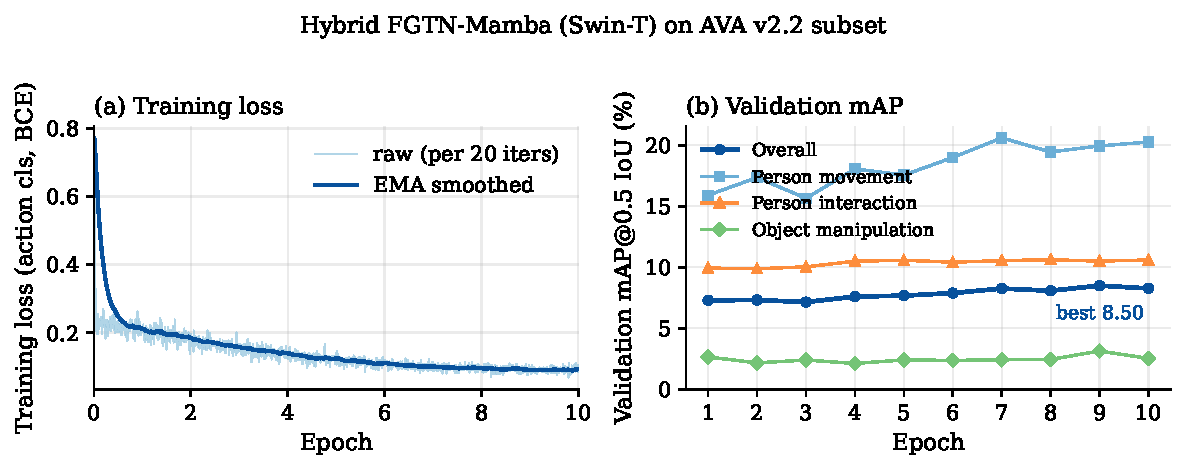
\includegraphics[width=\textwidth]{training_curves.pdf}
\caption[Đường cong huấn luyện và mAP kiểm định trên tập con AVA]{(a) Hàm mất mát huấn luyện (BCE) theo epoch, giá trị thô mỗi 20 iteration và đường làm mượt EMA. (b) mAP kiểm định tổng và theo ba nhóm hành vi; giá trị tốt nhất 8,50\% tại epoch~9. Vẽ từ \code{trainning.log}.}
\label{fig:curves}
\end{figure}

\begin{table}[htbp]
\centering
\caption{Tài nguyên của lần chạy trên tập con AVA với một GPU RTX~4090 (trích từ nhật ký)}
\label{tab:resources}
\begin{tabularx}{\textwidth}{lX}
\toprule
\textbf{Hạng mục} & \textbf{Giá trị}\\
\midrule
Số tham số & 41.827.383 (backbone 27.850.470; neck 13.914.624; head 62.289)\\
Bộ nhớ GPU đỉnh khi huấn luyện & 28.139 MB (epoch~1), 28.800 MB (epoch~2--10), lô 6, FP32\\
Bộ nhớ GPU đỉnh khi kiểm định & 2.058--2.838 MB, lô 1\\
Thời gian một iteration huấn luyện & 0,69--0,70 s (lô 6, gồm nạp dữ liệu 0,02 s)\\
Thời gian một mẫu kiểm định & 0,06--0,08 s (lô 1; $\approx 5{,}8$ phút cho 4.846 khung hình khóa)\\
Tổng thời gian 10 epoch & 5 giờ 55 phút, gồm huấn luyện và kiểm định\\
\bottomrule
\end{tabularx}
\end{table}

Ba nhóm hành vi của AVA có mức hiệu năng khác nhau rõ rệt và ổn định qua các epoch, phản ánh đúng các hạn chế đã nêu ở \cref{sec:gaps}:
\begin{itemize}
  \item \textbf{Chuyển động của người} (15,91\% $\rightarrow$ 20,61\%): tín hiệu toàn thân, bền vững theo thời gian, tương ứng các hành vi trạng thái trong phân xưởng như ngủ trên bàn, gác chân; nhóm được hưởng lợi nhiều nhất từ huấn luyện.
  \item \textbf{Tương tác giữa người} (9,94\% $\rightarrow$ 10,62\%): gần như không đổi sau epoch~4 vì phụ thuộc ngữ cảnh ngoài hộp người (L4), là động cơ tích hợp ACRN.
  \item \textbf{Thao tác với vật thể} (2,12--3,14\%): thấp nhất vì phụ thuộc vật thể nhỏ (L3) và nhiều lớp hiếm (L5), là động cơ cho đặc trưng đa tỉ lệ và hàm mất mát hai cấp; nhóm này cũng chịu ảnh hưởng nặng nhất của sai lệch tỷ lệ RoI dưới đây.
\end{itemize}

\label{sec:roi-stride}\textbf{Sai lệch tỷ lệ RoI.} Khi rà soát mã sau huấn luyện, luận văn phát hiện cấu hình của lần chạy này không đặt \code{featmap\_stride} cho \code{SingleRoIExtractor3D}, nên giá trị mặc định 16 được dùng trong khi tầng 4 của Video Swin-T có bước giảm mẫu 32. Hộp người vì vậy được ánh xạ lên bản đồ đặc trưng ở tỷ lệ gấp đôi: hộp ở nửa phải hoặc nửa dưới ảnh nhận đặc trưng bằng 0, hộp ở góc trên trái nhận đặc trưng của một vùng rộng gấp đôi. Sai lệch không ảnh hưởng tới nhận định về tính ổn định huấn luyện nhưng khiến giá trị mAP tuyệt đối không phản ánh đúng năng lực của cấu hình. Cấu hình một tỉ lệ đã được sửa thành \code{featmap\_stride = 32}; cấu hình đa tỉ lệ dùng 16, đúng với tầng 3 mà mọi bản đồ được nội suy về.

\section{Mốc tham chiếu trên AVA}
\label{sec:reference}

\Cref{tab:reference} liệt kê các mốc công bố trên AVA của những phương pháp ở \cref{ch:related} cùng hai số liệu của luận văn. Các mốc dùng giao thức, backbone và tiền huấn luyện khác nhau nên bảng chỉ cho thấy khoảng hiệu năng của bài toán; số liệu 8,50\% trên tập con không so sánh trực tiếp được với các mốc trên AVA đầy đủ.

\begin{table}[htbp]
\centering
\caption{Mốc công bố trên AVA và kết quả của luận văn (không so sánh trực tiếp; mức bằng chứng E4 cho các hàng tham chiếu)}
\label{tab:reference}
\small
\begin{tabularx}{\textwidth}{>{\raggedright\arraybackslash}p{3.9cm}>{\raggedright\arraybackslash}X>{\raggedright\arraybackslash}p{2.2cm}>{\raggedright\arraybackslash}X}
\toprule
\textbf{Phương pháp} & \textbf{Giao thức} & \textbf{mAP} & \textbf{Ghi chú}\\
\midrule
A* ngoại tuyến \cite{kim2024astar} & AVA v2.2, closed-set & 27,7 & SlowFast-R101-NL, Kinetics-600\\
STAR/CSN-152 \cite{gritsenko2024star} & AVA, end-to-end & 31,4 & IG65M $\to$ K400\\
STAR/B \cite{gritsenko2024star} & AVA, end-to-end & 30,0 & IN21K $\to$ K400\\
STAR/L \cite{gritsenko2024star} & AVA, end-to-end & 39,2 & CLIP $\to$ K700; 320 px\\
OV-STAD \cite{wu2024ovstad} & OV-AVA (base / novel / all) & 27,8 / 16,6 / 25,0 & Open-vocabulary\\
ST-CLIP \cite{huang2025stclip} & ZS-AVA (trung bình; với hộp thật) & 9,01 / 11,76 & Zero-shot\\
\midrule
Hybrid FGTN-Mamba (luận văn, hồ sơ thực nghiệm) & AVA v2.2, closed-set & 39,1 & Swin-T, K400; mức E2; \cref{sec:ava-record}\\
Swin-T + Hybrid FGTN-Mamba một tỉ lệ (luận văn, có nhật ký) & \textbf{Tập con} AVA v2.2, closed-set, \code{featmap\_stride} 16 & 8,50 & K400; 1 GPU; 10 epoch; \cref{sec:ava-subset}\\
\bottomrule
\end{tabularx}
\end{table}

\section{Trả lời câu hỏi nghiên cứu}
\label{sec:rq-answers}

\textbf{RQ1} --- Có cần temporal neck: có; ngay cả MHSA toàn cục tại vị trí hậu-backbone, tiền-RoI cũng tăng mAP ($+3{,}17$ / $+3{,}43$ điểm trên S1 / S2), nhưng Hybrid FGTN-Mamba còn cao hơn neck tiêu chuẩn đó 4,24 / 4,42 điểm. \textbf{RQ2} --- Quét hai chiều có ích ($+1{,}73$ / $+1{,}58$), hai nhánh bổ sung cho nhau ($+1{,}06$ / $+1{,}02$ so với Bi-SSM đứng riêng) và cổng sigmoid đóng góp thêm 1,76 / 1,85 điểm. \textbf{RQ3} --- Đa tỉ lệ cải thiện 3,85 / 2,00 điểm. \textbf{RQ4} --- ACRN cải thiện 5,89 / 3,90 điểm; phần hàm mất mát (A9) chưa có số liệu. \textbf{RQ5} --- Trả lời một phần: mọi thành phần vẫn có ích trên camera chưa thấy khi huấn luyện, với mAP của pipeline đầy đủ giảm từ 89,60\% xuống 78,15\%; số liệu 39,1 mAP trên AVA~v2.2 cần bổ sung cấu hình để đối chiếu.

\section{Hạn chế của nghiên cứu}
\label{sec:limitations}

\begin{itemize}
  \item \emph{Hàm mất mát và độ bất định}: ablation A9 chưa có số liệu; kết quả ablation chưa kèm độ lệch chuẩn giữa các hạt giống; các mô hình so sánh trong \cref{tab:main-results} là lượt chạy đơn, chưa đánh giá trên S2.
  \item \emph{Dữ liệu và tổng quát hóa}: bộ dữ liệu phân xưởng có số camera hạn chế; mAP của pipeline đầy đủ giảm 11,45 điểm khi chuyển sang camera mới; chưa có AP theo từng hành vi.
  \item \emph{Mức bằng chứng}: số liệu trên dữ liệu phân xưởng và 39,1 mAP trên AVA~v2.2 được tổng hợp từ hồ sơ thực nghiệm, nhật ký chi tiết chưa nằm trong kho mã; lần chạy trên tập con AVA còn sai lệch tỷ lệ RoI và learning rate chưa co giãn.
  \item \emph{Khoảng cách tới triển khai}: độ trễ đầu--cuối (gồm bộ phát hiện người và bộ đệm nhìn trước của quét hai chiều) chưa được đo; pipeline vẫn phụ thuộc person proposal và thiết lập closed-set.
\end{itemize}

\section*{Tiểu kết chương}
\addcontentsline{toc}{section}{Tiểu kết chương}

Trên bộ dữ liệu phân xưởng, pipeline đầy đủ đạt 89,83\% mAP và vượt các mô hình so sánh, với tốc độ trên 20 khung hình/giây. Ablation trên hai cách chia dữ liệu xác nhận đóng góp của temporal neck, của hai nhánh, của cổng sigmoid, của đặc trưng đa tỉ lệ và của ACRN; trong đó Hybrid FGTN-Mamba vượt neck tiêu chuẩn tại cùng vị trí hơn 4 điểm trên cả hai cách chia, đáp ứng tiêu chí chấp nhận đã đặt ra. Khoảng cách giữa S1 và S2 cho thấy 78,15\% trên camera mới là ước lượng thận trọng hơn cho triển khai. Các hạn chế về hàm mất mát, độ bất định và mức bằng chứng được nêu rõ để định hướng công việc tiếp theo.
